\documentclass[12pt]{article}
\usepackage{graphicx}
\usepackage{amsmath}
\usepackage{mathtools}
\usepackage{gensymb}
\usepackage[utf8]{inputenc}
\usepackage{float}
\usepackage{amssymb}
\newcommand{\mydet}[1]{\ensuremath{\begin{vmatrix}#1\end{vmatrix}}}
\providecommand{\brak}[1]{\ensuremath{\left(#1\right)}}
%\providecommand{\norm}[1]{\left\lVert#1\right\rVert}
\newcommand{\solution}{\noindent \textbf{Solution: }}
\renewcommand{\thefigure}{\thesection-\arabic{figure}}
\usepackage{tkz-euclide}
\usepackage[english]{babel}
\usepackage[utf8]{inputenc}
\usepackage[T1]{fontenc}
\usepackage{graphics}
\usepackage{standalone}
\usepackage{gensymb}
\usepackage{amsmath}
\newcommand{\myvec}[1]{\ensuremath{\begin{pmatrix}#1\end{pmatrix}}}
\let\vec\mathbf
\begin{document}
\begin{center}
\textbf\large{ STRAIGHT LINES}
\end{center}
\section*{Exercise 7.1}
Q3. AD and BC are equal perpendiculars to a line segment. Show that CD bisects AB.
\section*{Solution}

\begin{figure}[!h]
\begin{center}
\resizebox{0.3\linewidth}{!}
{
\documentclass{article}
\usepackage{tikz}
\usetikzlibrary{shapes.geometric,calc,angles,positioning,intersections,quotes,decorations,babel,patterns,fit}
\usepackage{tkz-euclide}
\begin{document}
\begin{tikzpicture}[scale =1.5,>=stealth,point/.style = {draw, circle, fill = black, inner sep = 1pt},]
\node (C) at (3,4)[point,label=above :$C$] {};
\node (O) at (0,0)[point,label=above :$O$] {};
\node (D) at (-3,-4)[point,label=below :$D$] {};
\node (B) at (0,4)[point,label=above :$B$] {};
\node (A) at (0,-4)[point,label=below :$A$] {};
\draw (A)--node[below] {$\textrm{a=4cm}$}(D);
\draw (A)--node[right] {$\textrm{c=3cm}$}(O);
\draw (D)--node[left] {$\textrm{b=5cm}$}(O);
\draw (B)--node[left] {$\textrm{c=3cm}$}(O);
\draw (B)--node[above] {$\textrm{a=4cm}$}(C);
\draw (O)--node[right] {$\textrm{b=5cm}$}(C);
\draw (A)--(O);
\draw (D)--(O);
\draw (O)--(C);
\draw (B)--(C);
\draw (O)--(B);
\tkzMarkAngle[fill=black!40,size=0.5cm,mark=](O,B,C)
\tkzMarkAngle[fill=black!40,size=0.5cm,mark=](O,A,D)

\end{tikzpicture}
\end{document}

}
\caption{Figure}
\label{fig:foo}
\end{center}
\end{figure}
Let
\begin{align}
    AD=a=4cm \\
    OA=c=3cm \\
    OD=b
\end{align}
Apply baudhayan theorem to find b for a triangle 
\begin{align}
    b^2=a^2+c^2\\
    b=\sqrt{a^2+c^2}=\sqrt{4^2+3^2}=5cm
\end{align}
\begin{itemize}
    \item  From the above figure,In $\triangle{BOC}$ and $\triangle{AOD}$ and from given information
\end{itemize}
    \begin{align}
    \angle BOC = \angle AOD 
    \label{eq:ang}\\
    \angle CBO = \angle DAO 
    \label{eq:ang2}\\
    BC=AD = b \\
    \therefore \triangle{BOC} \cong \triangle{AOD}\\
    \therefore OB=OA= c
    \end{align}
Thus, CD bisects AB and O is the mid-point of AB.
\begin{figure}[!h]
 \begin{center}
  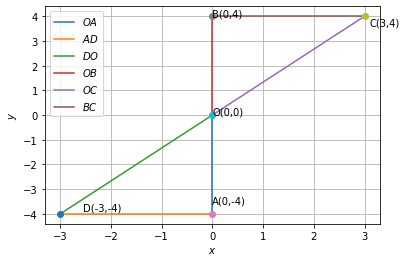
\includegraphics[width=\columnwidth]{./figs/python_fig.png}
 \end{center}
\caption{}
\label{fig:Python Generated Figure}
\end{figure}
\end{document}
